\documentclass[11pt]{article}
\usepackage[margin=0.82in]{geometry}
\usepackage[table]{xcolor}
\usepackage{tabularx}
\usepackage{array}
\usepackage{longtable}
\usepackage{booktabs}
\usepackage{enumitem}
\usepackage{parskip}
\usepackage{fancyhdr}
\usepackage{hyperref}
\usepackage{url}
\usepackage{graphicx}
\usepackage{float}
\hypersetup{colorlinks=true,linkcolor=black,urlcolor=blue,pdftitle={CraveDrop Security Assessment and Secure OIDC Login}}
\setlist[itemize]{noitemsep,topsep=3pt}
\setlist[enumerate]{noitemsep,topsep=3pt}
\setlength{\headheight}{14pt}
\setlength{\tabcolsep}{4pt}
\pagestyle{fancy}
\fancyhf{}
\lhead{CraveDrop Secure}
\rhead{Security assessment report}
\cfoot{\thepage}
\newcolumntype{Y}{>{\raggedright\arraybackslash}X}
\newcolumntype{P}[1]{>{\raggedright\arraybackslash}p{#1}}
\newcommand{\evidence}[1]{{\small\url{#1}}}
\emergencystretch=3em
\newcommand{\finding}[1]{\subsection{#1}}
\newcommand{\baseline}{\textbf{Baseline reproduction.} }
\newcommand{\impact}{\textbf{Impact.} }
\newcommand{\fix}{\textbf{Fix.} }
\newcommand{\control}{\textbf{Regression controls.} }
\newcommand{\residual}{\textbf{Residual risk.} }
\definecolor{tableblue}{HTML}{DCEAF4}

\begin{document}
\begin{titlepage}
\centering
\vspace*{1.3in}
{\Large SE4030 --- Secure Software Development\par}
\vspace{0.25in}
{\Huge\bfseries CraveDrop Security Assessment\par}
\vspace{0.12in}
{\Large and Secure OpenID Connect Customer Login\par}
\vspace{0.5in}
\rule{0.8\textwidth}{0.6pt}\par
\vspace{0.35in}
{\large Assignment report\par}
\vfill
\begin{tabular}{ll}
Hansaja A. M. G & IT22171856 \\
Dharmasiri I. D. N. D & IT22254320 \\
Sanjeewa P. D. L. B & IT22629708 \\
Aluthwaththa A. W. D. S. M & IT22267290 \\
\end{tabular}
\vfill
{\large September 2026\par}
\end{titlepage}

\pagenumbering{roman}
\tableofcontents
\clearpage
\pagenumbering{arabic}

\section{Executive summary}
This report presents a security assessment of CraveDrop, a food-ordering and delivery application implemented as microservices. The work preserves the original vulnerable source at immutable tag \evidence{baseline-vulnerable}, which resolves to commit \evidence{cb68a377f5b8cdc3b12f86883ac6fb703ef5e405}. The baseline was not altered.

The team identified, reproduced, fixed, and regression-tested seven distinct vulnerabilities. The findings cover missing authentication, object-level authorization, mass assignment, function-level authorization, payment workflow integrity, and token disclosure. Each counted finding has a different root cause. The evidence includes a redacted live baseline request, a focused code change, a blocked-attack check, and a legitimate authorized control. All seven demonstrated attack paths are blocked and all seven authorized controls remain usable. Remaining risks include signed payment confirmation, unassessed administration routes, XSS impact on cookie sessions, device/GPS integrity, WSO2 deployment trust material, and residual dependency/base-image maintenance.

The project also adds one customer-login feature using WSO2 Identity Server 7.1.0. It uses OpenID Connect Authorization Code flow with S256 PKCE. The application validates the identity token server-side and issues its own strict HttpOnly session cookies. This feature is separate from the seven counted vulnerabilities.

All fixtures are synthetic. No secrets, live customer data, bearer tokens, cookies, or unredacted logs are included in the repository or this report.

\section{Assignment alignment and project eligibility}
The assignment requires an application with sufficient scope, at least seven distinct vulnerabilities, fixes, discussion of remaining risks and preventive practices, an OAuth or OpenID Connect feature, and evidence of individual contribution. This report addresses those requirements as follows.

\begin{longtable}{P{0.29\linewidth}P{0.65\linewidth}}
\toprule
\rowcolor{tableblue}\textbf{Assignment requirement} & \textbf{Evidence in this submission} \\
\midrule
\endhead
Application scope and suitability & CraveDrop has separate user, order, payment, delivery, driver, restaurant, notification, email, and SMS components. It is a food-ordering application, not an intentionally vulnerable learning application. \\
Seven distinct vulnerabilities & Sections \ref{sec:findings} and \ref{sec:verification} describe V1--V7, their distinct root causes, before evidence, fixes, and controls. \\
OAuth or OpenID Connect feature & Section \ref{sec:oidc} documents a WSO2 OIDC customer login using Authorization Code with S256 PKCE. \\
Discussion and unfixed risks & Sections \ref{sec:remaining} and \ref{sec:prevention} list remaining vulnerabilities, reasons, and preventive practices. \\
Individual contribution & Section \ref{sec:contributions} maps allocated work to commits, tests, evidence, and the planned presentation segments. \\
\bottomrule
\end{longtable}

The original project is \href{https://github.com/nmdra/CraveDrop}{nmdra/CraveDrop} and uses the MIT licence. The selected default-branch baseline is dated 17 July 2025, before the July 2026 semester start. The modified repository is \href{https://github.com/nmdra/CraveDrop-Secure-SSD}{nmdra/CraveDrop-Secure-SSD}. The eligibility record is in \evidence{UPSTREAM.md} and \evidence{docs/eligibility-evidence.md}.

\section{Application scope and assessment method}
\subsection{Architecture and trust boundaries}
CraveDrop exposes a browser frontend through an NGINX gateway. The user service uses PostgreSQL. The order, payment, delivery, and driver services use separate service boundaries and databases. RabbitMQ supports asynchronous notification work. The assessment does not assume that gateway routing supplies authentication. Each changed controller or route checks identity and authorization at the relevant service boundary.

The principal types used in the tests are Customer A, Customer B, the assigned driver, and an unrelated driver. This makes the authorization checks reproducible without real personal data. Figure~\ref{fig:trust-boundaries} summarizes the boundary that each changed service enforces.

\begin{figure}[H]
  \centering
  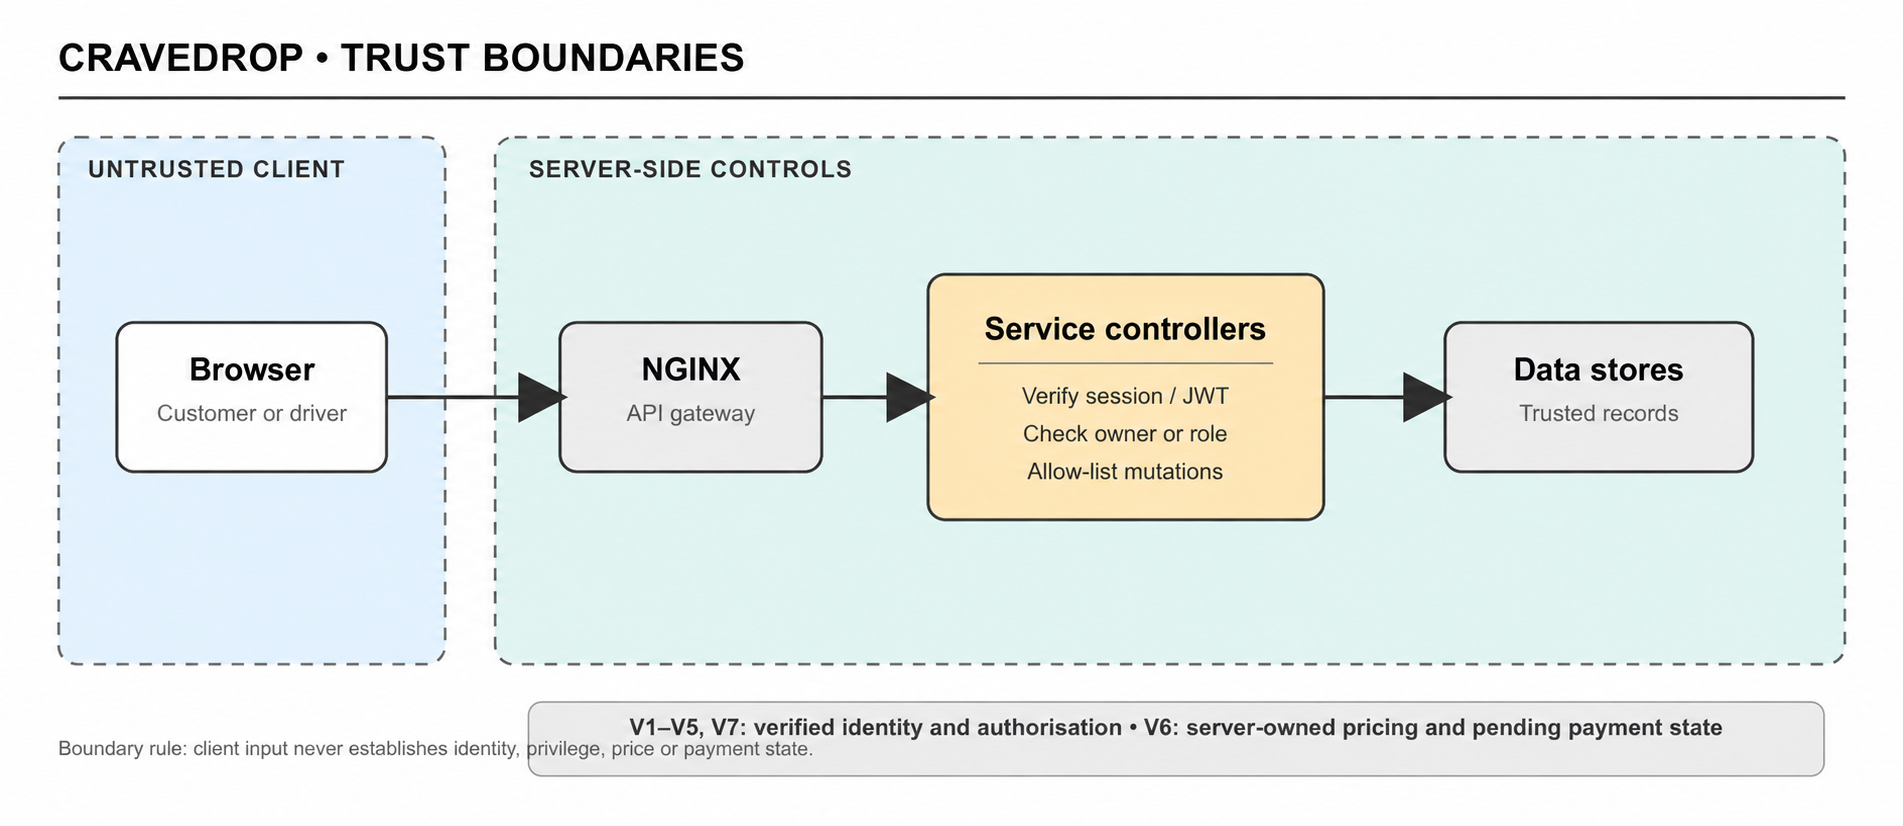
\includegraphics[width=0.92\linewidth]{assets/trust-boundaries-colored.png}
  \caption{CraveDrop client and service trust boundaries.}
  \label{fig:trust-boundaries}
\end{figure}

\subsection{Method}
The team used the following evidence-first procedure.
\begin{enumerate}
  \item Preserve the upstream source at \evidence{baseline-vulnerable}.
  \item Create deterministic synthetic A/B customer, driver, restaurant, product, order, and delivery fixtures.
  \item Run a redacted live HTTP attack against the baseline.
  \item Apply the smallest focused fix that preserves a valid authorized path.
  \item Run a negative regression test and a positive authorized control.
  \item Link the evidence, test, and fix commit in \evidence{docs/finding-matrix.md}.
\end{enumerate}

A 401 or 403 response alone does not establish a complete fix. Each test also proves that an authorized synthetic principal can use the protected function.

\subsection{Scope limits}
The assessment counts only V1--V7. Delivery and notification BOLA variants were retained as backup observations, not counted as extra findings. Dependency advisories from \texttt{npm audit} are also not counted without a reproduced application impact. This avoids reporting multiple URLs with the same root cause as separate vulnerabilities.

\section{Finding summary}\label{sec:findings}
\begin{longtable}{P{0.055\linewidth}P{0.25\linewidth}P{0.22\linewidth}P{0.38\linewidth}}
\toprule
\rowcolor{tableblue}\textbf{ID} & \textbf{Finding} & \textbf{Classification} & \textbf{Verified secure result} \\
\midrule
\endhead
V1 & Missing payment authentication & CWE-306; OWASP API2 & Anonymous payment actions return 401; an authenticated customer reaches the payment-start handler. \\
V2 & Order IDOR/BOLA & CWE-639; OWASP API1 & A foreign customer cannot read the other customer's order; the owner can. \\
V3 & Order mass assignment & CWE-915; OWASP API3 & Client attempts to set protected order fields return 400; valid authorized actions work. \\
V4 & Unauthorized delivery mutation & CWE-862; OWASP API5 & Only the assigned driver can make allowed status and location updates. \\
V5 & Broken driver administration authorization & CWE-862; OWASP API5 & A driver can update own availability, not another driver's. \\
V6 & Payment amount and state manipulation & CWE-841; API business logic & The server calculates the amount and creates a pending order despite tampered values. \\
V7 & Sensitive token disclosure and session design & CWE-922, CWE-532; OWASP API2 & No bearer token is returned in JSON, stored in browser storage, or logged. \\
\bottomrule
\end{longtable}

\finding{V1: Missing authentication on payment actions}
\baseline An anonymous request to \evidence{POST /api/payments/create-payment-intent} reached the payment handler. It did not receive an authentication error. The redacted live response is \evidence{evidence/V1-before.txt}.

\impact An unauthenticated actor could invoke a payment action, consume payment-provider resources, and bypass the intended customer boundary.

\fix Payment routes now require a verified Bearer JWT. The service derives the caller identity from the verified token rather than request input.

\control The same anonymous action returns 401. An authenticated synthetic customer reaches the payment-start handler. The local Stripe test configuration rejects the request after authorization, which proves the authorization boundary but not a real card charge. See \evidence{evidence/V1-after.txt}, \evidence{security-tests/runtime-v1-v3.mjs}, commits \evidence{4dc9756} and \evidence{720a077}.

\residual Stripe configuration and provider-side controls remain necessary. This assessment does not process a live card charge.

\finding{V2: Order insecure direct object reference}
\baseline An unauthenticated request read Customer A's synthetic order by order ID. The request returned the order record. See \evidence{evidence/V2-before.txt}.

\impact An attacker who knows or obtains an order ID could read or modify another customer's order.

\fix Order reads and mutations now require an authenticated customer. The controller scopes the order query to both the requested order ID and the verified customer ID.

\control Customer B receives 404 when requesting Customer A's order. Customer A can read the owned order. Evidence is \evidence{evidence/V2-after.txt}; the runtime control is \evidence{security-tests/runtime-v1-v3.mjs}; the commits are \evidence{4dc9756} and \evidence{720a077}.

\residual The order ID remains an identifier. Every future order route must preserve the ownership scope.

\finding{V3: Order mass assignment}
\baseline An unauthenticated order update supplied \evidence{userId}, \evidence{totalAmount}, \evidence{status}, and \evidence{createdAt}. The baseline persisted these client-controlled fields. See \evidence{evidence/V3-before.txt}.

\impact A caller could alter ownership, price, lifecycle state, or audit data.

\fix The controller rejects protected fields and allow-lists only supported customer-editable fields. The server owns order identity, price, payment state, and timestamps.

\control A payload containing protected fields returns 400. A valid authorized update and order creation succeed. See \evidence{evidence/V3-after.txt}, \evidence{security-tests/runtime-v1-v3.mjs}, commits \evidence{4dc9756} and \evidence{720a077}.

\residual A new editable field must undergo explicit review before it is added to the allow-list.

\finding{V4: Unauthorized delivery mutation}
\baseline An anonymous request changed a delivery status, and the same boundary accepted driver-location changes. The baseline evidence is \evidence{evidence/V4-before.txt}.

\impact An attacker could falsify delivery progress or tracking data.

\fix Delivery writes require a valid driver JWT, an assigned-driver identity match, and an allow-listed status transition.

\control Anonymous, customer, and unrelated-driver writes fail. The assigned driver can make the demonstrated valid status and location updates. A reverse transition returns 409. See \evidence{evidence/V4-after.txt}, \evidence{security-tests/runtime-v4-v7.mjs}, \evidence{security-tests/regression-v4-v7.mjs}, commits \evidence{c84ec0a} and \evidence{132f768}.

\residual The service does not prove the integrity of a driver device or GPS source.

\finding{V5: Broken driver administration authorization}
\baseline An unauthenticated request changed Driver B's availability by using Driver B's URL identifier. See \evidence{evidence/V5-before.txt}.

\impact An attacker could disrupt delivery allocation and service availability.

\fix Driver availability updates now require a valid driver JWT. The verified driver ID must match the URL driver ID.

\control One driver cannot update another driver's availability. A driver can update own availability. See \evidence{evidence/V5-after.txt}, \evidence{security-tests/runtime-v4-v7.mjs}, \evidence{security-tests/regression-v4-v7.mjs}, commits \evidence{c84ec0a} and \evidence{132f768}.

\residual This finding covers driver availability only. Restaurant administration requires separate review before it can be claimed as protected.

\finding{V6: Payment amount and state manipulation}
\baseline A client created a card order with \evidence{totalAmount=1} instead of the synthetic trusted total of 2500. The baseline also marked the order paid. See \evidence{evidence/V6-before.txt}.

\impact A customer could reduce the payable amount or obtain a paid order without confirmed payment.

\fix The order service calculates the USD total from trusted product data. It ignores client currency and paid-status fields. New card orders start in the pending state.

\control Tampered amount, currency, and payment-state values do not control the persisted order. The test persists 2500 USD and pending state. An authenticated customer can create a server-priced order. See \evidence{evidence/V6-after.txt}, \evidence{security-tests/runtime-v4-v7.mjs}, \evidence{security-tests/regression-v4-v7.mjs}, commits \evidence{c84ec0a} and \evidence{132f768}.

\residual A future confirmation path must bind a trusted order to a verified payment-provider event.

\finding{V7: Sensitive token disclosure and session design}
\baseline Login and refresh responses returned bearer tokens in JSON. User-service logs recorded refresh-token data, and the browser stored access tokens. See \evidence{evidence/V7-before.txt}.

\impact Script injection, browser access, log access, or log forwarding could disclose bearer tokens and enable session impersonation.

\fix Login and refresh now issue credentialed strict HttpOnly cookies. The frontend no longer stores bearer tokens. Request logging records the request path but omits query values, which also prevents OIDC authorization-code logging. Cookie mutations require the approved Origin.

\control Login and refresh JSON omit access tokens. Browser storage and application logs do not contain bearer tokens. A missing or wrong Origin blocks cookie mutation. An approved-origin session can access profile and refresh operations. See \evidence{evidence/V7-after.txt}, \evidence{security-tests/runtime-v4-v7.mjs}, \evidence{security-tests/regression-v4-v7.mjs}, commits \evidence{c84ec0a} and \evidence{132f768}.

\residual HttpOnly cookies reduce token theft but do not prevent a successful XSS attack from making same-origin requests while a session exists.

\section{Verification and reproducibility}\label{sec:verification}
\subsection{Fixtures and baseline integrity}
The deterministic fixture definition is \evidence{security-tests/fixtures/security-fixtures.json}. The reset command writes ignored active fixture data with local-only permissions. The team verified the fixture contents before runtime checks. Baseline attacks ran in a separate worktree checked out at the immutable tag.

\subsection{Test evidence}
\begin{longtable}{P{0.08\linewidth}P{0.26\linewidth}P{0.28\linewidth}P{0.29\linewidth}}
\toprule
\rowcolor{tableblue}\textbf{Area} & \textbf{Before evidence} & \textbf{After evidence} & \textbf{Focused checks} \\
\midrule
\endhead
V1--V3 & \evidence{evidence/V1-before.txt} through \evidence{V3-before.txt} & \evidence{evidence/V1-after.txt} through \evidence{V3-after.txt} & \evidence{security-tests/runtime-v1-v3.mjs} \\
V4--V7 & \evidence{evidence/V4-before.txt} through \evidence{V7-before.txt} & \evidence{evidence/V4-after.txt} through \evidence{V7-after.txt} & \evidence{runtime-v4-v7.mjs} and \evidence{regression-v4-v7.mjs} \\
OIDC & Not a baseline vulnerability & \evidence{evidence/oidc-after.txt} & \evidence{regression-oidc.mjs} and \evidence{oidc-mocked.mjs} under Node 20 \\
\bottomrule
\end{longtable}

The source-contract checks verify that the security controls remain in the changed routes and services. The runtime checks verify the HTTP behavior. The evidence files are redacted. They do not contain credentials, complete tokens, or cookies. A fresh clean clone built the Compose stack, passed the V1--V7 runtime and source checks, and recreated the documented WSO2 client and synthetic user for a real callback and protected-session control.

\subsection{Supporting tools}
The team ran \texttt{npm audit} against the user, order, payment, delivery, and driver services. The commands, tool versions, and severity counts are recorded in \evidence{evidence/tools/npm-audit.txt}. These advisories are dependency-maintenance input, not counted application vulnerabilities, because no endpoint impact was reproduced.

The team completed a local OWASP ZAP 2.17.0 passive scan on 2026-09-18. It used the headless package launcher, a conventional bounded spider, and passive rules against only \url{http://127.0.0.1:5000}. It made no active attack, authenticated request, WSO2 request, direct-service request, database request, RabbitMQ request, or external request. The initial scan returned three medium and six low alert instances. The instances reduced to two shared gateway-hardening causes: missing CSP headers on fallback responses and Nginx version disclosure in fallback content and the \texttt{Server} header. The gateway now sets a CSP and disables Nginx version tokens. A verification scan reported zero missing-CSP-header and version-disclosure alerts, with three remaining medium CSP policy-completeness alerts. No application exploit was reproduced and no counted vulnerability was added. See \evidence{evidence/tools/zap-summary.md}.

The team also ran Trivy 0.68.2 vulnerability-only scans on a fresh source export and the Compose images. The initial source scan returned 6 critical, 123 high, 163 medium, and 28 low dependency findings. The initial image scan returned 20 critical and 395 high alert instances. After the selected compatible dependency updates, the final source scan returned 0 critical, 32 high, 72 medium, and 21 low findings. The final image scan covered 14 artifacts and returned 16 critical, 357 high, 358 medium, 144 low, and 18 unknown alert instances. These are per-artifact totals, not unique-CVE totals, because dependencies and base-image packages repeat across images. See \evidence{evidence/tools/trivy-summary.md}.

The initial critical inventory included \href{https://nvd.nist.gov/vuln/detail/CVE-2025-44005}{CVE-2025-44005}, \href{https://nvd.nist.gov/vuln/detail/CVE-2025-68121}{CVE-2025-68121}, \href{https://nvd.nist.gov/vuln/detail/CVE-2025-7783}{CVE-2025-7783}, \href{https://nvd.nist.gov/vuln/detail/CVE-2026-30836}{CVE-2026-30836}, \href{https://nvd.nist.gov/vuln/detail/CVE-2026-31789}{CVE-2026-31789}, \href{https://nvd.nist.gov/vuln/detail/CVE-2026-33186}{CVE-2026-33186}, and \href{https://nvd.nist.gov/vuln/detail/CVE-2026-59873}{CVE-2026-59873}. These NVD URLs are record/lookup citations; Trivy's package, version, artifact and reachability triage remains authoritative for this run, and none is a reproduced V1--V7 application finding.

The selected remediation updated vulnerable \texttt{form-data}, Axios, Mongoose, React Router, and the application bcrypt/tar path. The selected findings were absent from the final source and image checks. Remaining scanner results include base-image and unrelated dependency maintenance risks, including \texttt{tar} in the Node base-image npm layer. These results do not prove that an untrusted request reaches a vulnerable function, so they do not add an eighth application vulnerability. The full triage record is \evidence{docs/security-tool-triage.md}.

\section{WSO2 OpenID Connect customer login}\label{sec:oidc}
\subsection{Feature objective}
The added feature provides one customer sign-in path through WSO2 Identity Server 7.1.0. It does not add account linking, role synchronization, or automated logout. The intent is to demonstrate a secure OpenID Connect grant implementation without exposing provider tokens to the browser.

\subsection{Security design}
The user service creates cryptographically random state, nonce, and PKCE verifier values. It sends the S256 challenge to WSO2 and stores the temporary flow in a signed, short-lived, HttpOnly cookie. The callback compares state before token exchange, exchanges the authorization code server-side, and validates the provider issuer, client audience, RS256 signature, expiry, nonce, and subject.

The local CraveDrop account key is the provider issuer plus subject. The service explicitly rejects automatic local-account linking by matching an email address. The local WSO2 test user store released only a subject claim. In that controlled case, the service keeps the issuer-plus-subject binding and stores a deterministic non-deliverable \evidence{@identity.invalid} placeholder rather than assuming an email address. Figure~\ref{fig:wso2-flow} shows the server-side exchange and validation sequence.

\begin{figure}[H]
  \centering
  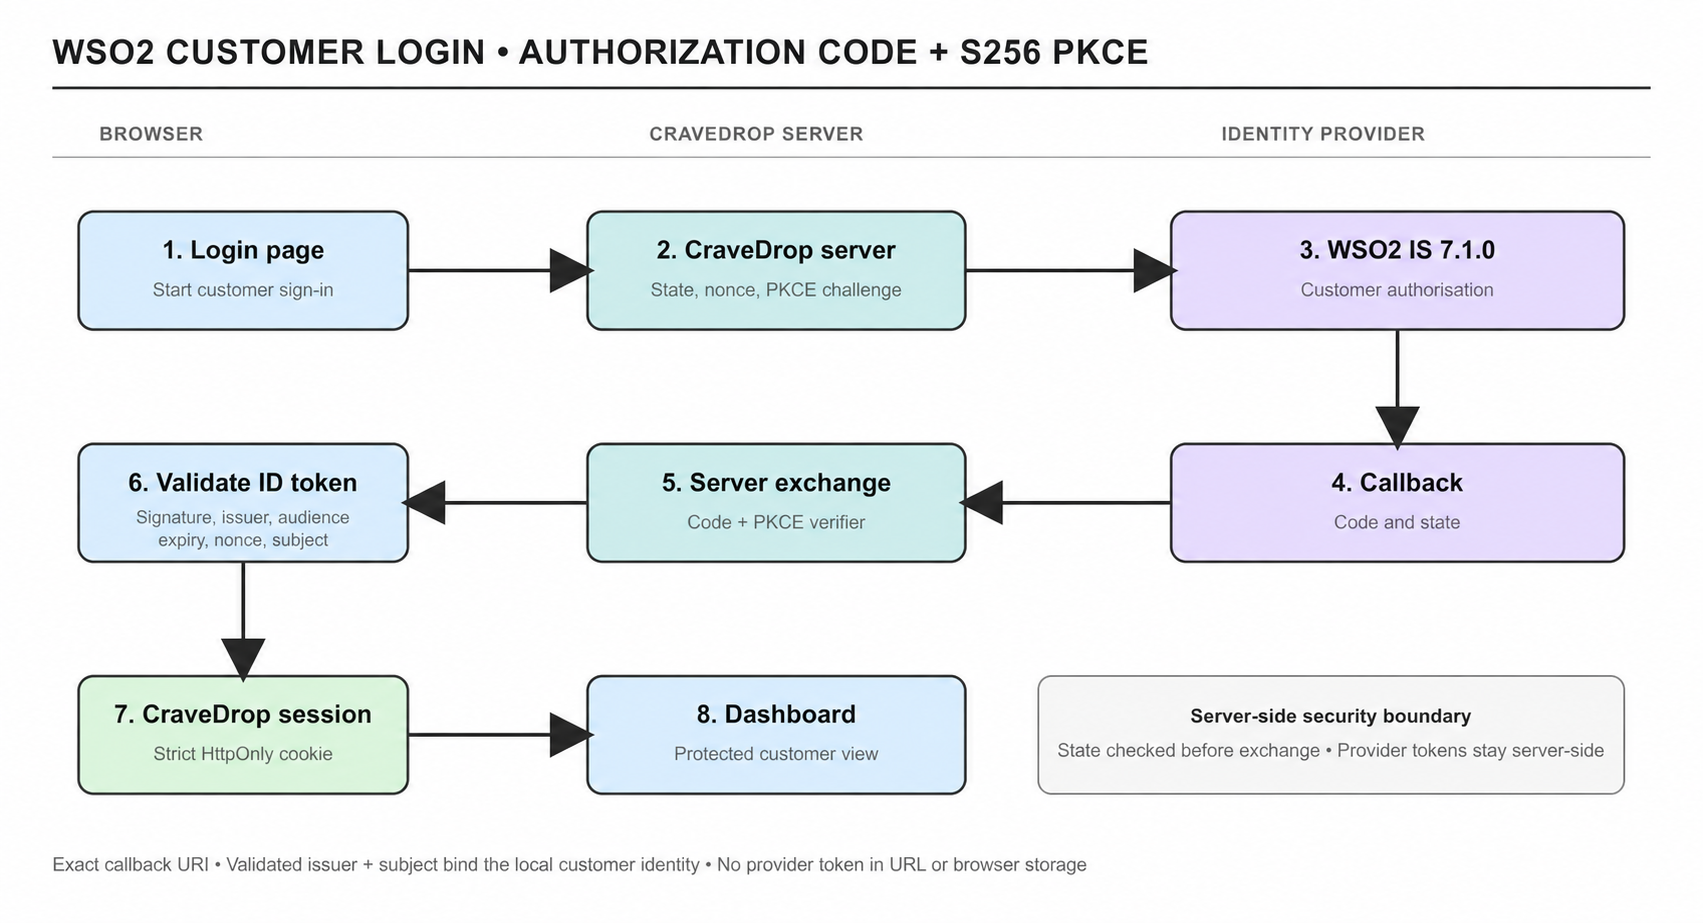
\includegraphics[width=0.90\linewidth]{assets/wso2-oidc-colored.png}
  \caption{WSO2 Identity Server customer-login flow.}
  \label{fig:wso2-flow}
\end{figure}

\subsection{Feature verification}
A synthetic WSO2 customer completed a real local flow. The callback returned HTTP 302 to an allow-listed dashboard path, issued strict HttpOnly CraveDrop session cookies, expired the temporary flow cookie, and authorized a protected validation endpoint. No provider token appeared in the callback URL.

The mocked Node 20 suite confirms that a tampered state is rejected before token exchange and that an invalid nonce or identity token is rejected. The proof is \evidence{evidence/oidc-after.txt}; the tests are \evidence{security-tests/regression-oidc.mjs} and \evidence{security-tests/oidc-mocked.mjs}; the implementation commit is \evidence{28e178c}.

\section{Remaining vulnerabilities and limitations}\label{sec:remaining}
The following risks were identified but are not claimed as fixed or counted as additional vulnerabilities.

\begin{longtable}{P{0.27\linewidth}P{0.30\linewidth}P{0.35\linewidth}}
\toprule
\rowcolor{tableblue}\textbf{Risk or limitation} & \textbf{Reason not fixed in this scope} & \textbf{Recommended follow-up} \\
\midrule
\endhead
Restaurant administration controls & The seven-findings scope uses driver availability for V5. Restaurant routes need an independent assessment and test set. & Review each restaurant mutation for verified role and ownership checks. \\
Notification BOLA variants & These share an authorization root cause with other object-access findings. Counting them would inflate the seven-finding portfolio. & Assess them separately and add principal-scoped notification access. \\
XSS impact on cookie sessions & HttpOnly prevents token reads but not same-origin actions initiated by injected script. & Review CSP coverage and output encoding, then add XSS tests. \\
Payment confirmation integration & The local control demonstrates trusted order state, not a real payment-provider confirmation. & Verify signed provider webhooks and bind each event to the trusted order and amount. \\
Driver device and GPS integrity & API authorization cannot verify the physical source of a reported location. & Apply mobile/device controls and anomaly detection where appropriate. \\
Gateway response hardening & The ZAP verification scan retains three medium CSP policy-completeness alerts. No exploit was reproduced. & Review the remaining CSP directives and confirm compatibility with the frontend and API routes. \\
Dependency and base-image CVEs & Trivy still reports base-image and unrelated dependency findings after the selected compatible updates. Package reachability and exploitability are not established. & Review base images and remaining advisories in a separate maintenance task. Do not treat them as V1--V7 without reproduction. \\
\bottomrule
\end{longtable}

\section{Discussion and preventive secure software engineering practices}\label{sec:prevention}
The observed vulnerabilities are preventable through routine engineering controls.
\begin{itemize}
  \item \textbf{Threat modelling at route design.} Define the actor, resource owner, permitted action, and server-owned state before implementing a route.
  \item \textbf{Authorization as a service-boundary contract.} Verify identity from a signed token or session. Do not derive identity or privilege from body, query, or URL data alone.
  \item \textbf{Allow-list mutation inputs.} Accept only fields required by the user action. Compute prices, account IDs, payment state, and audit timestamps on the server.
  \item \textbf{Security regression tests.} Keep an attack test and an authorized control for every authorization and state-change rule.
  \item \textbf{Secure session engineering.} Keep bearer credentials out of JSON, browser storage, URLs, and logs. Use strict HttpOnly cookies with origin checks for cookie-mutating requests.
  \item \textbf{Dependency and configuration review.} Review audit output, container configuration, default credentials, logging, and environment handling. Do not treat an advisory as an exploit without impact evidence.
  \item \textbf{Evidence hygiene.} Use synthetic fixtures, redact captures, and ensure secret-bearing files are ignored before commits, reports, and videos.
\end{itemize}

\section{Individual contributions}\label{sec:contributions}
The repository records work in coherent commits. The final video must show each member explaining the allocated work. The team will not manufacture commits solely to increase contribution counts.

\begin{longtable}{P{0.25\linewidth}P{0.17\linewidth}P{0.49\linewidth}}
\toprule
\rowcolor{tableblue}\textbf{Member} & \textbf{Registration number} & \textbf{Allocated work and evidence} \\
\midrule
\endhead
Hansaja A. M. G & IT22171856 & User-session and token hardening, WSO2 OIDC login, \evidence{28e178c}, \evidence{evidence/oidc-after.txt}, and OIDC video segment. \\
Dharmasiri I. D. N. D & IT22254320 & Order authentication, BOLA, mass-assignment controls, \evidence{4dc9756}, \evidence{720a077}, and V1--V3 video segments. \\
Sanjeewa P. D. L. B & IT22629708 & Delivery and driver authorization, payment integrity, \evidence{c84ec0a}, \evidence{132f768}, and V4--V6 video segments. \\
Aluthwaththa A. W. D. S. M & IT22267290 & Synthetic fixtures, \evidence{ced39e3}, tool evidence, report material, README, submission packaging, and video segments. \\
\bottomrule
\end{longtable}

\section{Conclusion}
CraveDrop now has seven independently evidenced security fixes and a secure WSO2 OIDC customer-login feature. The work preserves a reproducible vulnerable baseline and verifies both blocked attacks and legitimate authorized flows. The report records completed ZAP and Trivy scans, selected compatible remediation, and residual scanner risks without presenting scanner alerts as application exploits or extra counted findings. The final submission must add the unlisted video URL to \evidence{README.txt}, regenerate the final ZIP, and upload it to CourseWeb.

\begin{thebibliography}{9}
\bibitem{assignment} SE4030, \textit{Secure Software Development Assignment}, 2026. Provided assignment brief.
\bibitem{owasp-api} OWASP Foundation, \textit{OWASP API Security Top 10}. \url{https://owasp.org/www-project-api-security/}
\bibitem{owasp-top10} OWASP Foundation, \textit{OWASP Top 10 Web Application Security Risks}. \url{https://owasp.org/www-project-top-ten/}
\bibitem{cwe} MITRE, \textit{Common Weakness Enumeration}. \url{https://cwe.mitre.org/}
\bibitem{oidc} OpenID Foundation, \textit{OpenID Connect Core 1.0}. \url{https://openid.net/specs/openid-connect-core-1_0.html}
\bibitem{rfc7636} IETF, \textit{RFC 7636: Proof Key for Code Exchange by OAuth Public Clients}. \url{https://www.rfc-editor.org/rfc/rfc7636}
\bibitem{wso2} WSO2, \textit{WSO2 Identity Server Documentation}. \url{https://is.docs.wso2.com/}
\end{thebibliography}

\section*{Appendix A: Complete OWASP ZAP passive scan report}
\addcontentsline{toc}{section}{Appendix A: Complete OWASP ZAP passive scan report}
\textbf{Scope.} Initial and verification scans were completed on 18 September 2026 in the local lab with OWASP ZAP 2.17.0. The package launcher was \texttt{/usr/share/zaproxy/zap.sh -daemon}. The target was \url{http://127.0.0.1:5000}. Each run used a conventional spider with \texttt{maxChildren=10}, followed by passive scanning. Active scanning, authentication, WSO2, direct service ports, databases, RabbitMQ, and external URLs were excluded. Both runs exited with status 0. The system wrapper \texttt{/usr/bin/zaproxy} starts the GUI; it was not used for the recorded headless runs.

\textbf{Initial result counts.} Three Medium alert instances de-duplicated to one missing Content-Security-Policy cause on gateway fallback responses. Six Low instances de-duplicated to one Nginx version-disclosure cause in fallback content and the \texttt{Server} header. High: 0. Informational: 0. The affected paths were \,\texttt{/}, \texttt{/robots.txt}, and \texttt{/sitemap.xml}; direct local requests confirmed the initial observations.

\textbf{Remediation and verification.} The gateway now sets \texttt{server\_tokens off} and applies the policy \texttt{default-src 'self'; base-uri 'self'; frame-ancestors 'none'; object-src 'none'}. The verification scan found zero missing-CSP-header alerts and zero Nginx version-disclosure alerts. It retained three Medium \textit{CSP: Failure to Define Directive with No Fallback} instances on the same paths. The header is present; the residual alert concerns policy completeness, not absence of a policy. No application exploit was reproduced and no V8 finding was added.

\textbf{Evidence handling.} Complete JSON reports, response data, and daemon logs remain local in \texttt{/tmp/cravedrop-zap-20260918-152734} and \texttt{/tmp/cravedrop-zap-final-20260918T113513Z}. They are not committed because scanner output can contain response data. The committed summary contains no cookies, authorization headers, codes, tokens, or personal data.

\clearpage
\section*{Appendix B: Complete Trivy CVE scan report}
\addcontentsline{toc}{section}{Appendix B: Complete Trivy CVE scan report}
\textbf{Scope.} Initial and verification scans used Trivy 0.68.2 in the pinned \texttt{aquasec/trivy:0.68.2} image with vulnerability scanning only. Secret, misconfiguration, licence, and active network scanning were excluded. Unfixed findings were included; neither run used \texttt{--ignore-unfixed}. The initial target was a fresh source clone without a runtime \texttt{.env}; the verification target was a clean working-tree export with ignored runtime files and \texttt{node\_modules} excluded. The initial image set contained 13 Compose images; the verification set contained those 13 plus the separately maintained restaurant-service image.

\textbf{Initial counts.} The source scan returned Critical 6, High 123, Medium 163, and Low 28. The 13-image scan returned 20 Critical and 395 High alert instances. Image counts are per artifact and include duplicate CVEs; they must not be summed as a unique-CVE total.

\textbf{Initial per-artifact image counts.}
\begin{longtable}{P{0.38\linewidth}P{0.50\linewidth}}
\toprule
\rowcolor{tableblue}\textbf{Artifact} & \textbf{Counts (Critical / High / Medium / Low / Unknown)} \\
\midrule
\endhead
\texttt{mongo:7.0} & 1 / 96 / 70 / 18 / 9 \\
\texttt{nginx:alpine} & 0 / 36 / 70 / 37 / 6 \\
\texttt{nmdra/delivery-service} & 1 / 10 / 7 / 1 / 0 \\
\texttt{nmdra/driver-service} & 2 / 18 / 10 / 1 / 0 \\
\texttt{nmdra/email-service} & 1 / 14 / 20 / 4 / 0 \\
\texttt{nmdra/frontend} & 6 / 75 / 74 / 42 / 2 \\
\texttt{nmdra/notification-service} & 1 / 15 / 17 / 3 / 0 \\
\texttt{nmdra/order-service} & 1 / 10 / 7 / 1 / 0 \\
\texttt{nmdra/payment-service} & 1 / 10 / 7 / 1 / 0 \\
\texttt{nmdra/sms-service} & 2 / 25 / 29 / 4 / 0 \\
\texttt{nmdra/user-service} & 3 / 54 / 39 / 7 / 0 \\
\texttt{postgres:17-alpine} & 1 / 30 / 28 / 14 / 1 \\
\texttt{rabbitmq:4-management-alpine} & 0 / 2 / 6 / 12 / 0 \\
\bottomrule
\end{longtable}

\textbf{Initial critical-CVE inventory.} The seven candidates below are scanner observations, not reproduced CraveDrop exploits. The linked labels are NVD record/lookup citations; Trivy's package, installed-version, artifact, and reachability analysis remains authoritative for this run.

\begin{longtable}{P{0.25\linewidth}P{0.27\linewidth}P{0.16\linewidth}P{0.23\linewidth}}
\toprule
\rowcolor{tableblue}\textbf{CVE citation} & \textbf{Package/version} & \textbf{Fixed version} & \textbf{Affected artifact} \\
\midrule
\endhead
\href{https://nvd.nist.gov/vuln/detail/CVE-2025-44005}{CVE-2025-44005} & \texttt{github.com/}\newline\texttt{smallstep/certificates 0.26.1} & 0.29.0 & Frontend image \\
\href{https://nvd.nist.gov/vuln/detail/CVE-2025-68121}{CVE-2025-68121} & Go standard library 1.24.2/1.24.6 & 1.24.13, 1.25.7, or 1.26.0-rc.3 & Frontend and infrastructure images \\
\href{https://nvd.nist.gov/vuln/detail/CVE-2025-7783}{CVE-2025-7783} & \texttt{form-data 4.0.2} & 4.0.4 & SMS image and source scan \\
\href{https://nvd.nist.gov/vuln/detail/CVE-2026-30836}{CVE-2026-30836} & \texttt{github.com/}\newline\texttt{smallstep/certificates 0.26.1} & 0.30.0 & Frontend image \\
\href{https://nvd.nist.gov/vuln/detail/CVE-2026-31789}{CVE-2026-31789} & \texttt{libcrypto3/libssl3 3.3.4-r0} & 3.3.7-r0 & Frontend image \\
\href{https://nvd.nist.gov/vuln/detail/CVE-2026-33186}{CVE-2026-33186} & \texttt{google.golang.org/grpc 1.67.1} & 1.79.3 & Frontend image \\
\href{https://nvd.nist.gov/vuln/detail/CVE-2026-59873}{CVE-2026-59873} & \texttt{tar 6.2.1/7.5.11} & 7.5.19 & Node service images and source tree \\
\bottomrule
\end{longtable}

\begin{sloppypar}
\textbf{Applied compatible remediation.} The gateway received CSP and \texttt{server\_tokens off}. Application dependency resolutions updated \texttt{form-data} to 4.0.6, Axios to 1.20.0, Mongoose to 8.24.4, React Router to 7.18.2, and bcrypt to 6.0.0 in the affected user and driver services. The source regression, service rebuilds, and verification rescans passed. The selected Axios, form-data, Mongoose, and React Router findings were absent from final results, as was the application \texttt{tar} 6.2.1 path.
\end{sloppypar}

\textbf{Verification counts and residual risk.} The final source export returned Critical 0, High 32, Medium 72, and Low 21. The verification scan over 14 artifacts returned 16 Critical, 357 High, 358 Medium, 144 Low, and 18 Unknown alert instances. A remaining \texttt{tar} 7.5.11 finding is in the bundled npm layer of the \texttt{node:22-alpine} base image. Base-image upgrades were outside the approved scope, so this remains a dependency-maintenance risk rather than a reproduced application vulnerability. No CVE was promoted to V8 or another counted finding; the assignment portfolio remains V1--V7.

\textbf{Evidence handling.} Raw JSON, image digests, and the clean clone remain in local mode-0700 directories recorded in \evidence{evidence/tools/trivy-summary.md}; they are not submission artifacts. The source exports excluded runtime \texttt{.env} files, active fixture data, and \texttt{node\_modules}.

\end{document}
